\documentclass{article}
\usepackage[utf8]{inputenc}
\usepackage{hyperref}
\usepackage{listings}
\usepackage{multimedia} % to embed movies in the PDF file
\usepackage{graphicx}
\usepackage{comment}
\usepackage[english]{babel}
\usepackage{amsmath}
\usepackage{amsfonts}
\usepackage{wrapfig}
\usepackage{multirow}
\usepackage{verbatim}
\usepackage{float}
\usepackage{cancel}
\usepackage{caption}
\usepackage{subcaption}
\usepackage{mathdots}
\usepackage[margin=1.25 in]{geometry}
\usepackage{/home/cade/Homework/latex-defs}
\usepackage{/home/cade/Homework/jlcode}

\title{AMATH 586 Final}
\author{Cade Ballew \#2120804}
\date{June 7, 2022}

\begin{document}
	
\maketitle
	
\section{Problem 1}
We consider the ODE 

\begin{align*} v'(t) = \frac 1 \epsilon g(v(t)), \quad g(v) = v (\alpha - v) (1-v) - w. \end{align*}

which we solve numerically using the TR-BDF-2 method,

\[U^* = U^n + \frac k 4 (f(U^n) + f(U^*)),\\
U^{n+1} = \frac 1 3 \left( 4 U^* -U^n + k f(U^{n+1})\right),\]
in Julia. Using \(v(0) = 0.3\), \(\alpha= 0.5\),
\(w = 0.1\) and \(\epsilon = 0.01\) as the parameters, we observe the following solution when solving to $t=0.1$ with a stepsize of $k=10^{-5}$. \\
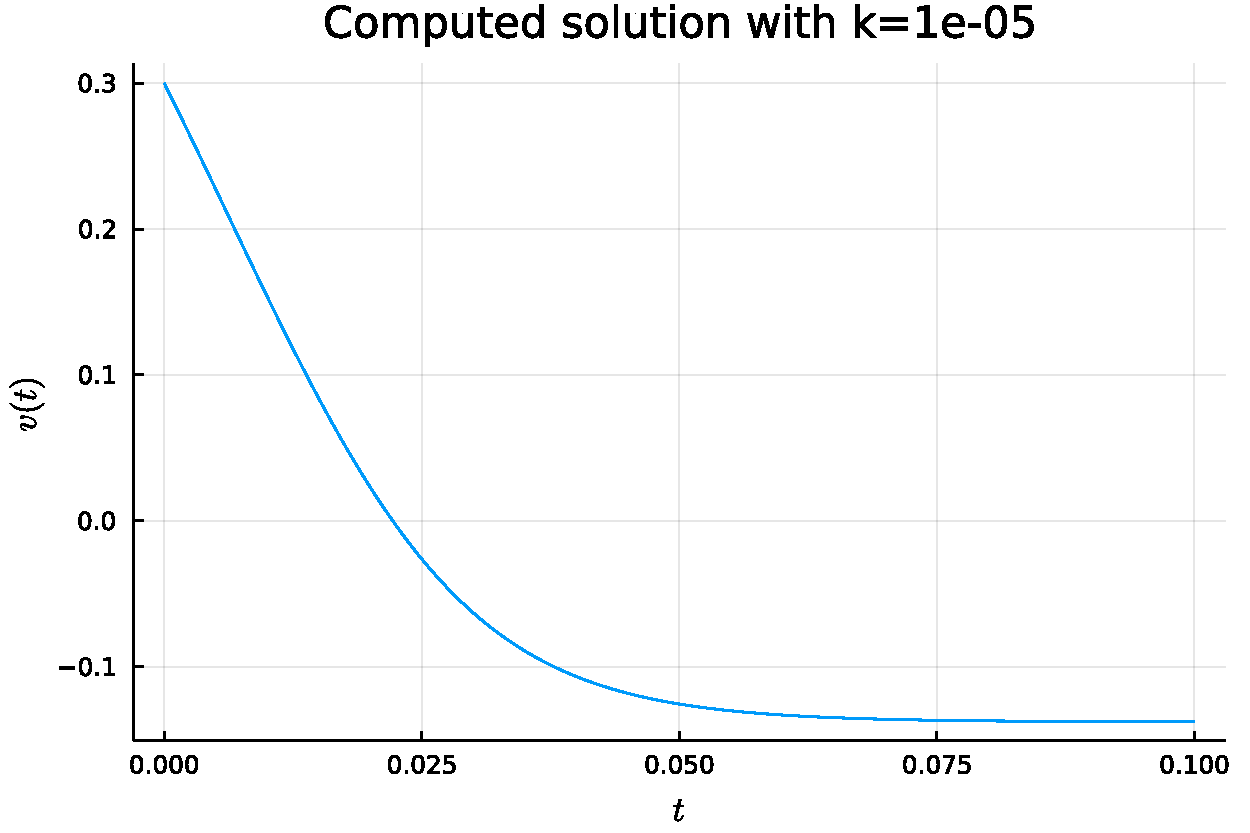
\includegraphics[scale=0.5]{prob1.pdf}\\
To verify that our method is indeed second order accurate at $t=0.1$, we treat the value that we found with this stepsize of $k=10^{-5}$ as the true solution and compute the error and reduction ratio $$\frac{\text{Error with time step } 2k}{\text{Error with time step } k}$$ for $k=2^{-j}$ where $j=4,\ldots,10$. Doing this, our Julia code prints the following table. 
\begin{verbatim}
    t      |      error       | reduction ratio 
6.2500e-03 | 8.6012600408e-06 | 
3.1250e-03 | 2.1200162577e-06 | 4.0571670191e+00
1.5625e-03 | 5.2458346345e-07 | 4.0413326105e+00
7.8125e-04 | 1.3036374619e-07 | 4.0239980730e+00
3.9063e-04 | 3.2473860656e-08 | 4.0144209390e+00
1.9531e-04 | 8.0895766474e-09 | 4.0142843157e+00
9.7656e-05 | 2.0048369631e-09 | 4.0350296789e+00
\end{verbatim}
For an $r$th-order method we should see this be approximately $2^r$, so this suggests that our method is indeed second order as most of our values are approximately 4.
 
\section{Problem 2}
Now, we consider the ODE system \begin{align*} v'(t) &= \frac 1 \epsilon \left( g(v(t)) - w(t) + I_a \right), \quad g(v) = v (\alpha - v) (1-v),\\
	w'(t) &= \beta v(t) - \gamma w(t)\end{align*}
by writing the system as

\begin{align*}
	\begin{bmatrix} v'(t) \\ w'(t) \end{bmatrix} = \mathcal A\left(\begin{bmatrix} v(t) \\ w(t) \end{bmatrix} \right) + \mathcal B\left(\begin{bmatrix} v(t) \\ w(t) \end{bmatrix} \right)
\end{align*} where \begin{align*}
	\mathcal A \left(\begin{bmatrix} v \\ w \end{bmatrix} \right) &= \begin{bmatrix} \frac 1 \epsilon \left( g(v) - w+ I_a \right) \\ 0\end{bmatrix}, \\
	\mathcal B \left(\begin{bmatrix} v \\ w \end{bmatrix} \right) &= \begin{bmatrix} 0 \\ \beta v - \gamma w\end{bmatrix}
\end{align*}
and solve the problem numerically by Strange splitting, applying TR-BDF-2 to $\mathcal{A}$ and RK2 to $\mathcal{B}$. Taking \begin{align*} \alpha = 0.3, \quad \beta = 1, \quad I_a = 0, \quad \epsilon = 0.001,
\end{align*}
with initial data

\begin{align*}
v(0) = v_0, \quad w(0) = 0,
\end{align*}
we observe the following when $v_0=0.31$ with small timestep $k=10^{-5}$ and run until time $t=1$. \\
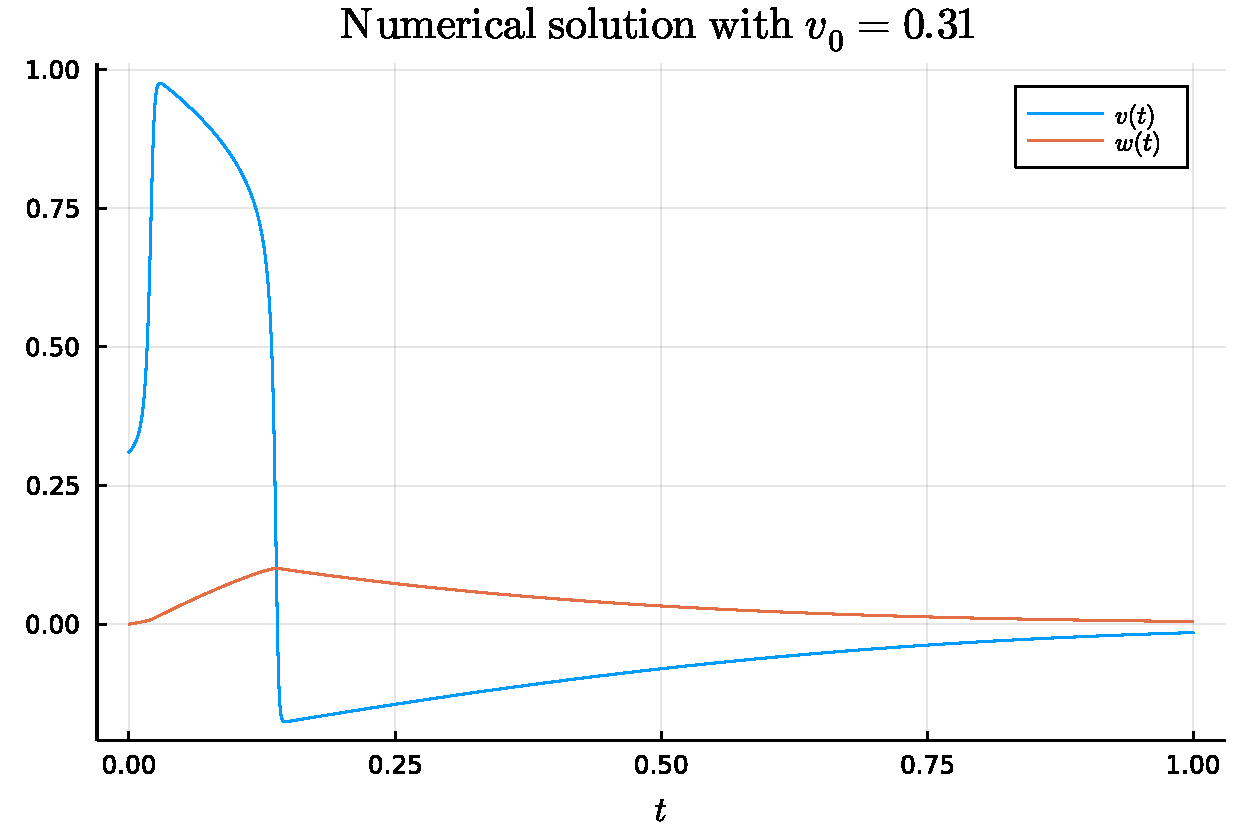
\includegraphics[scale=0.5]{prob2a.pdf}\\
If we instead take $v_0=0.29$ and run to time $t=0.25$, we observe the following.\\
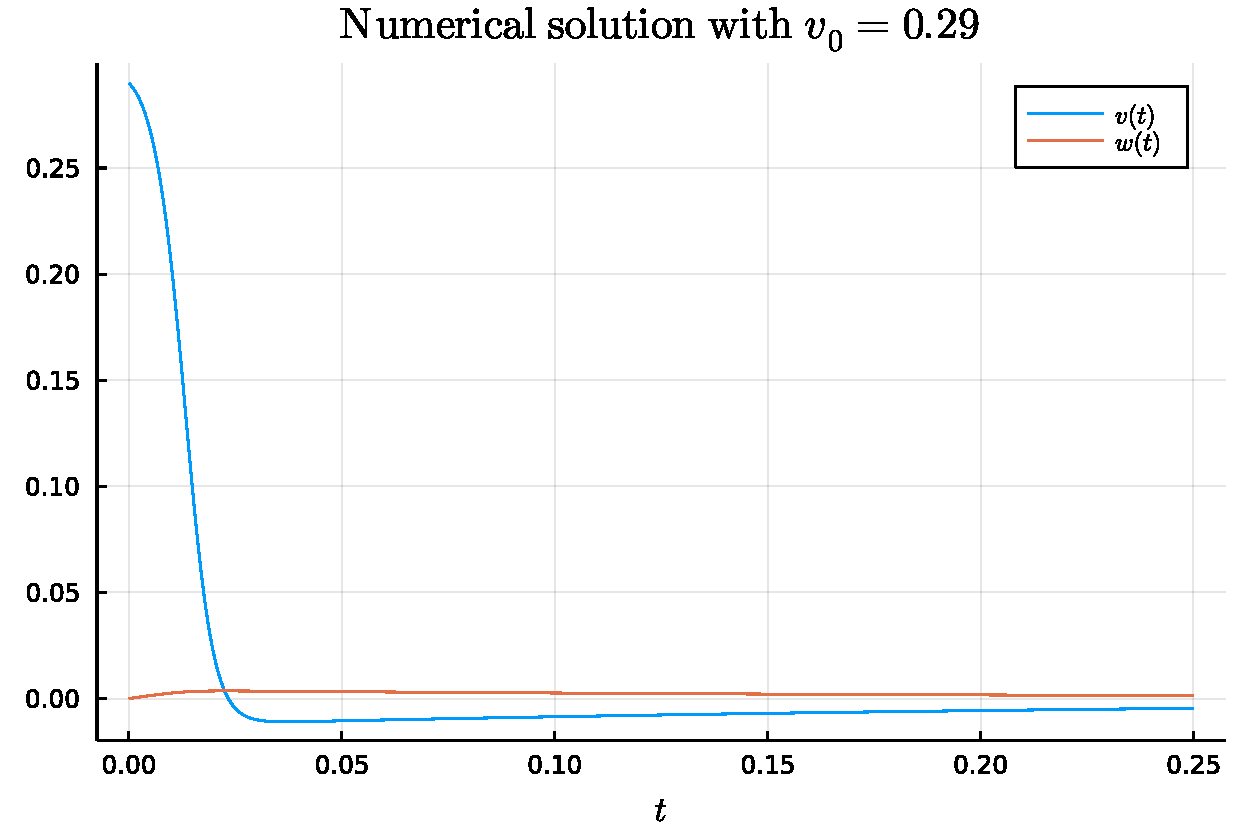
\includegraphics[scale=0.5]{prob2b.pdf}\\
To verify that our method is indeed second order accurate at $t=0.25$ with this choice of initial condition, we treat the value that we found with this stepsize of $k=10^{-5}$ as the true solution and compute the error and reduction ratio $$\frac{\text{Error with time step } 2k}{\text{Error with time step } k}$$ for $k=2^{-j}$ where $j=4,\ldots,10$ for both $v$ and $w$. Doing this, our Julia code prints the following table. 
\begin{verbatim}
    t      |     error v      |     error w      |reduction ratio v |reduction ratio w
6.2500e-03 | 1.2097180179e-04 | 3.9611015529e-05 |
3.1250e-03 | 3.2088976949e-05 | 1.0536269722e-05 | 3.7698865246e+00 | 3.7594914115e+00
1.5625e-03 | 8.1769070508e-06 | 2.6897904284e-06 | 3.9243416551e+00 | 3.9171340676e+00
7.8125e-04 | 2.0594483574e-06 | 6.7813039540e-07 | 3.9704355885e+00 | 3.9664796721e+00
3.9063e-04 | 5.1631333772e-07 | 1.7009814519e-07 | 3.9887568399e+00 | 3.9867007053e+00
1.9531e-04 | 1.2902289893e-07 | 4.2517400749e-08 | 4.0017186253e+00 | 4.0006713062e+00
9.7656e-05 | 3.2025072342e-08 | 1.0554730014e-08 | 4.0288089765e+00 | 4.0282793301e+00
\end{verbatim}
For an $r$th-order method we should see this be approximately $2^r$, so this suggests that our method is indeed second order as most of our values are approximately 4 for both $v$ and $w$.\\
Finally, we set $I_a=0.2$ and $v_0=0$ and obtain the following plot.\\
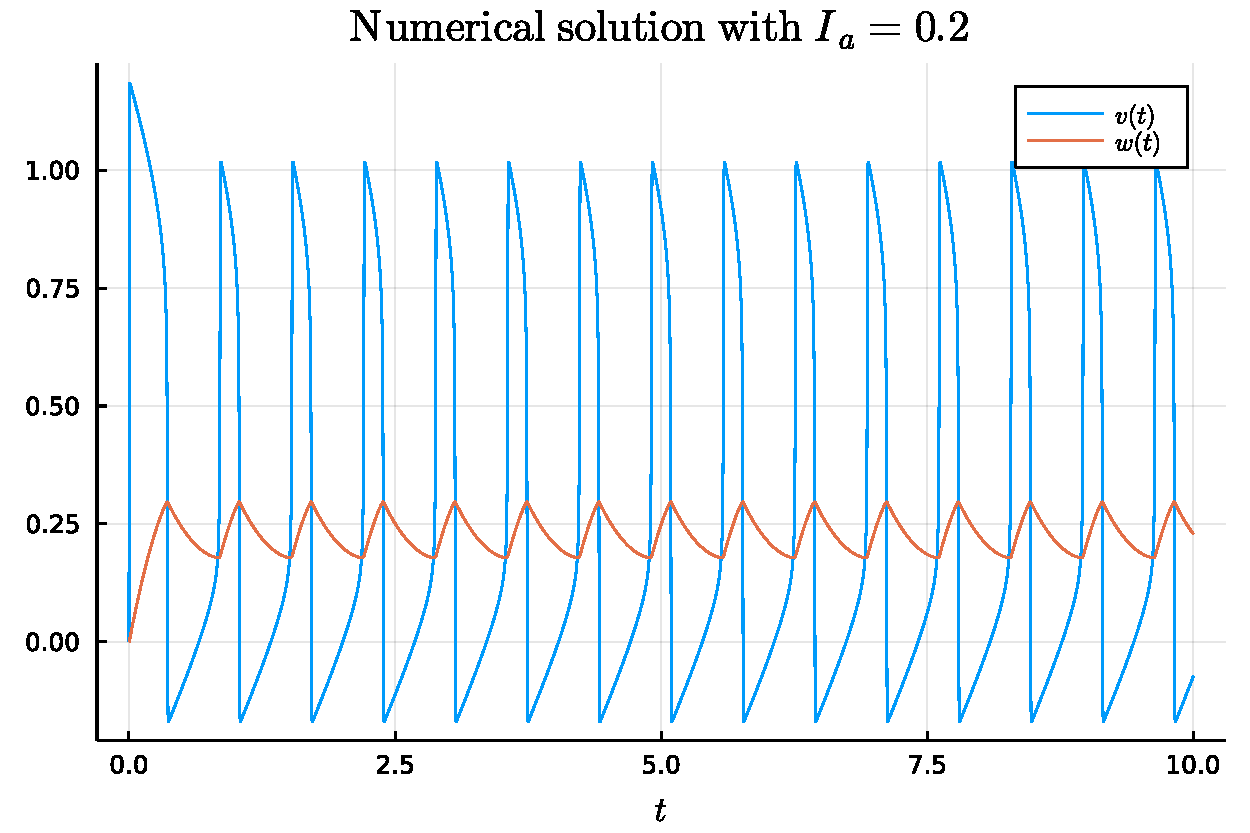
\includegraphics[scale=0.5]{prob2c.pdf}

\section{Problem 3}
Now, we consider the heat equation

\begin{align*}
	v_t = \kappa v_{xx}, \quad t > 0,\quad x \in (a,b).
\end{align*}
with Neumann boundary conditions \(v_x(a,t) = 0 = v_x(b,t)\) which has MOL discretization
\begin{align*}
	V'(t) = \frac{\kappa}{h^2} A V(t),
\end{align*}

where

\begin{align*}
	V(t) = \begin{pmatrix} V_0(t)\\ V_1(t) \\ \vdots \\ V_{m+1}(t) \end{pmatrix},
\end{align*}

and

\begin{align*}
	A = \begin{pmatrix}
		-2  & 2\\
		1 & -2 & 1 \\
		& 1 & -2 & 1\\
		&& \ddots & \ddots & \ddots \\
		&&& 1 & -2 & 1\\
		&&&& 2 & -2 \end{pmatrix}.
\end{align*}
We apply TR-BDF-2 to this discretization where $a=0$, $b=4$, and initial data 
\begin{align*}
	v(x,0) = \begin{cases} 1 &a \leq x < \frac{a+b}{2} \\
		0 & \text{otherwise}.
	\end{cases}
\end{align*}
Taking \(h = 0.01\), \(k = h\) and \(\kappa = 1\), we solve this problem numerically to time $t=6$. In the following, we display the computed solution at each integral time. 
\begin{figure}[H]
	\centering
	\begin{subfigure}{0.3\linewidth}
		\centering
		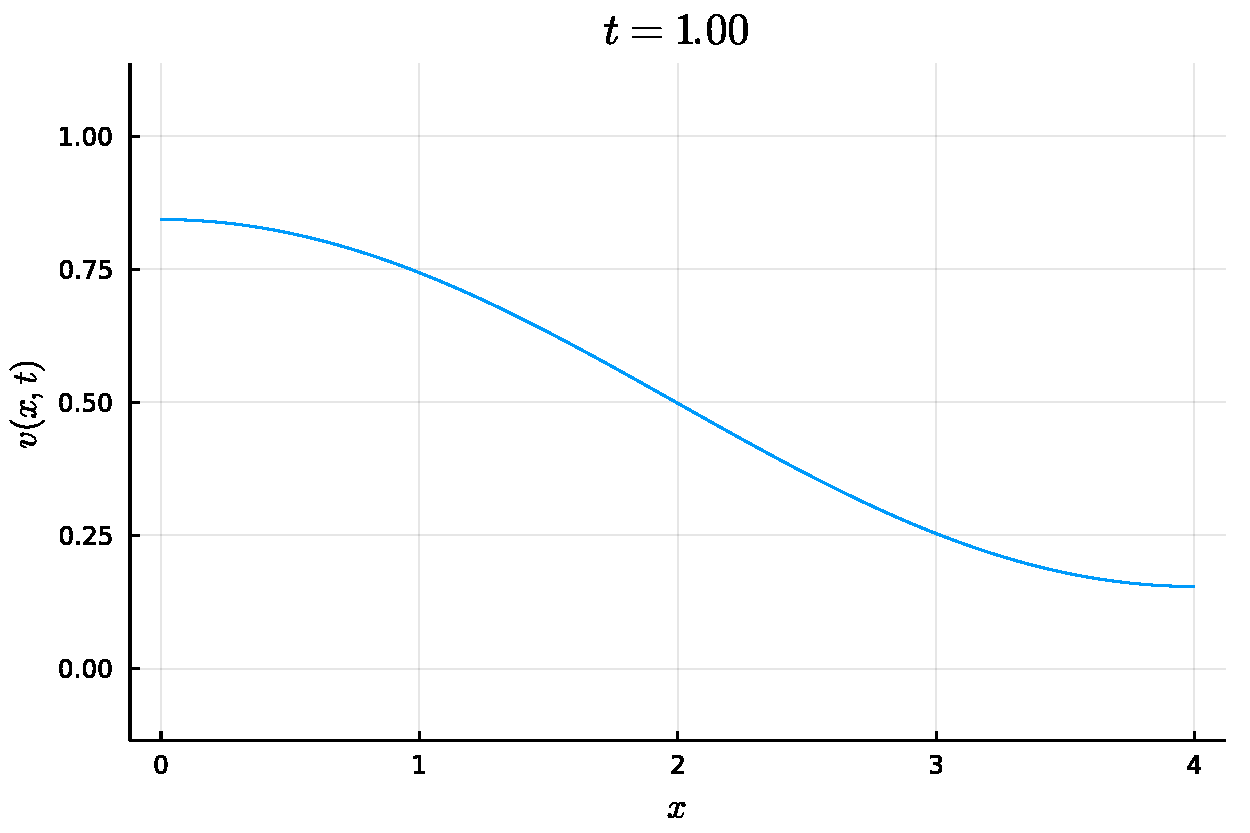
\includegraphics[width=\linewidth]{prob3_t=1.pdf}
	\end{subfigure}
	\begin{subfigure}{0.3\linewidth}
		\centering
		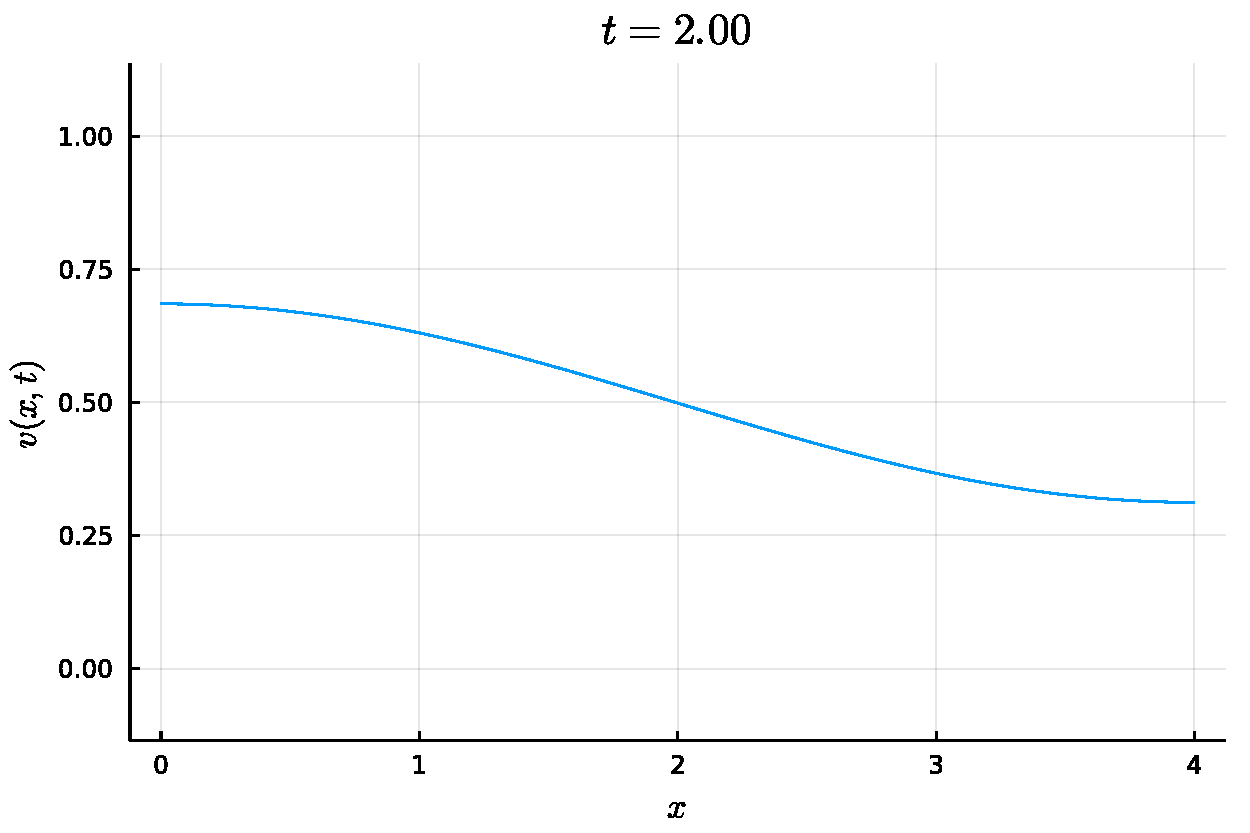
\includegraphics[width=\linewidth]{prob3_t=2.pdf}
	\end{subfigure}
	\begin{subfigure}{0.3\linewidth}
		\centering
		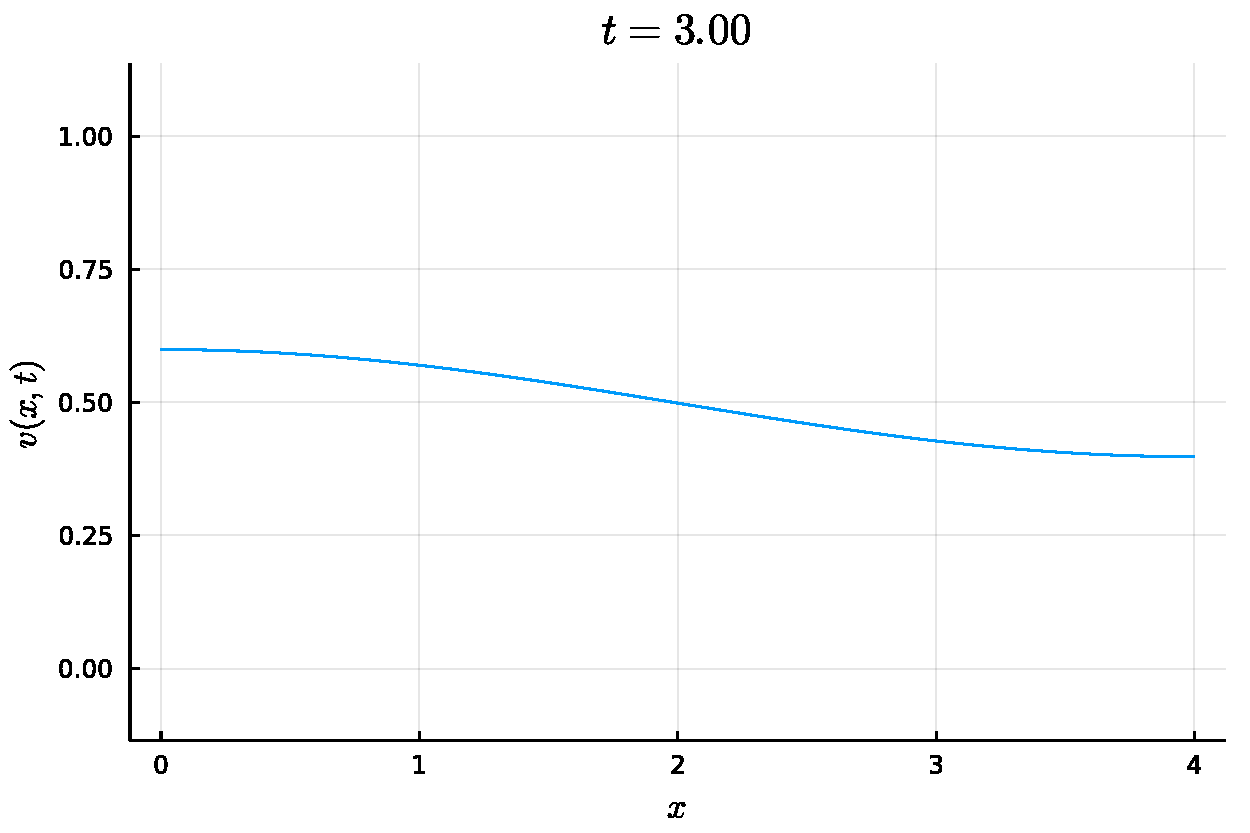
\includegraphics[width=\linewidth]{prob3_t=3.pdf}
	\end{subfigure}
	\begin{subfigure}{0.3\linewidth}
		\centering
		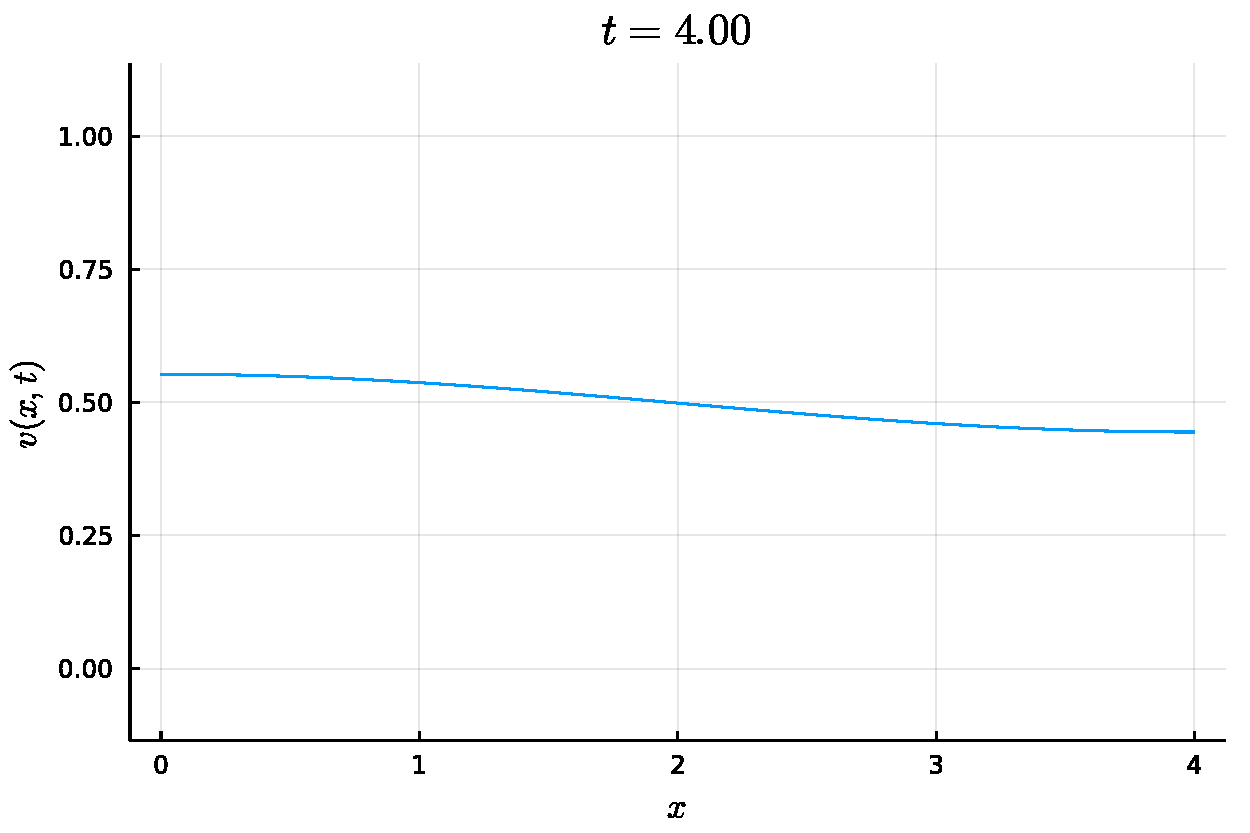
\includegraphics[width=\linewidth]{prob3_t=4.pdf}
	\end{subfigure}
	\begin{subfigure}{0.3\linewidth}
		\centering
		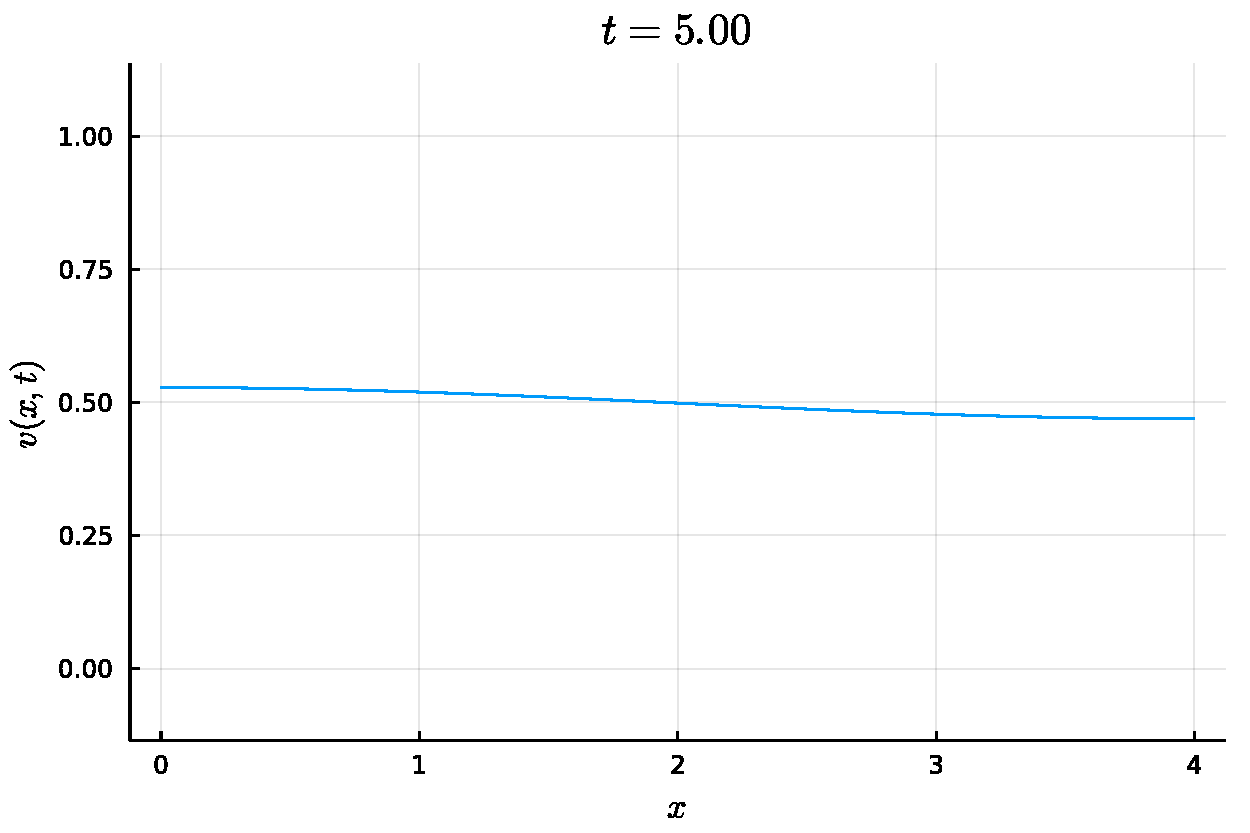
\includegraphics[width=\linewidth]{prob3_t=5.pdf}
	\end{subfigure}
	\begin{subfigure}{0.3\linewidth}
		\centering
		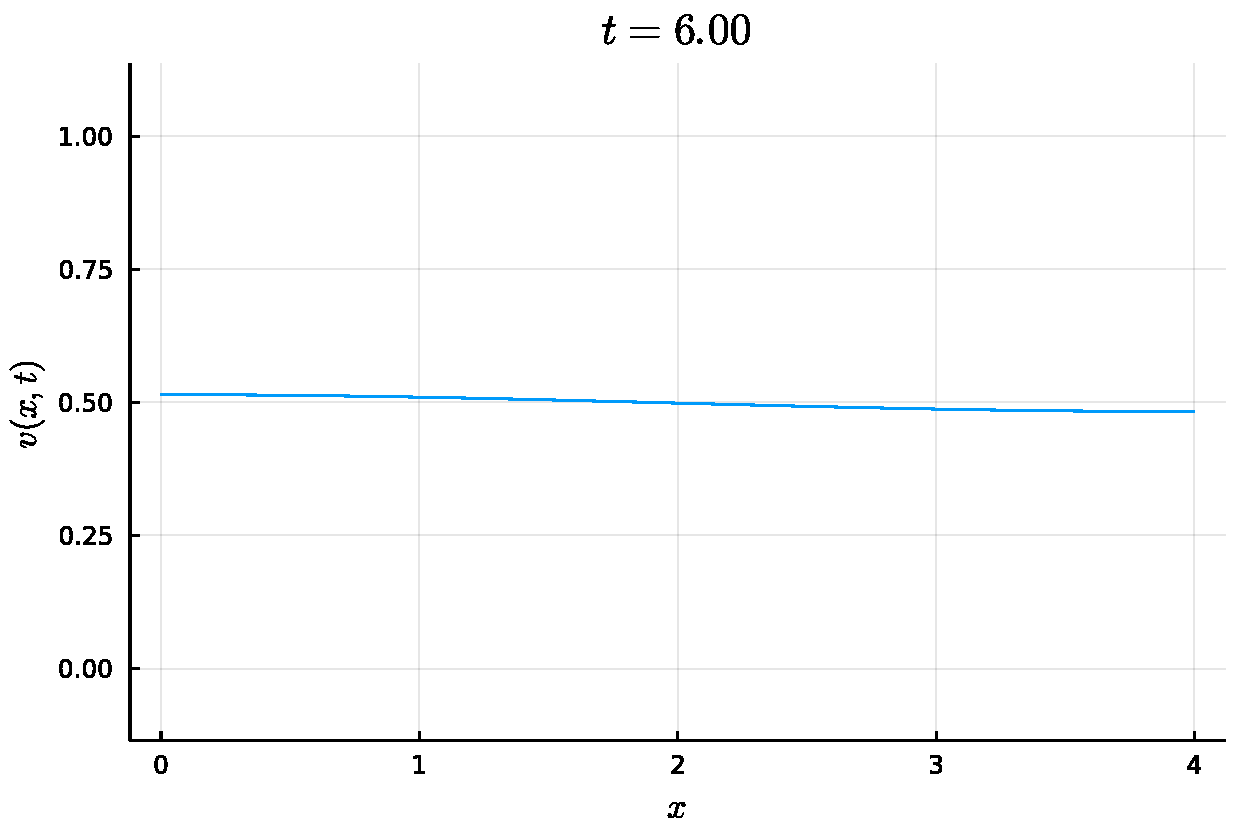
\includegraphics[width=\linewidth]{prob3_t=6.pdf}
	\end{subfigure}
\end{figure}
We also include the following \href{https://imgur.com/a/E9uNlVp}{gif} of the computed solution over time.\\
While this solution appears to be converging to the long-time limit \(v(x,t) \approx 1/2\) as \(t \to \infty\), there is actually a small discrepancy between the numerical behavior and our expectation that the integral of the solution be nearly preserved. This would imply that the integral should be approximately $2$ at each timestep, but if we plot the difference between the average value of our computed solution scaled by $k$\footnote{I.e., the $1$ grid-norm minus $2$} (so that it is an approximation to the integral) and this, we observe the following.\\
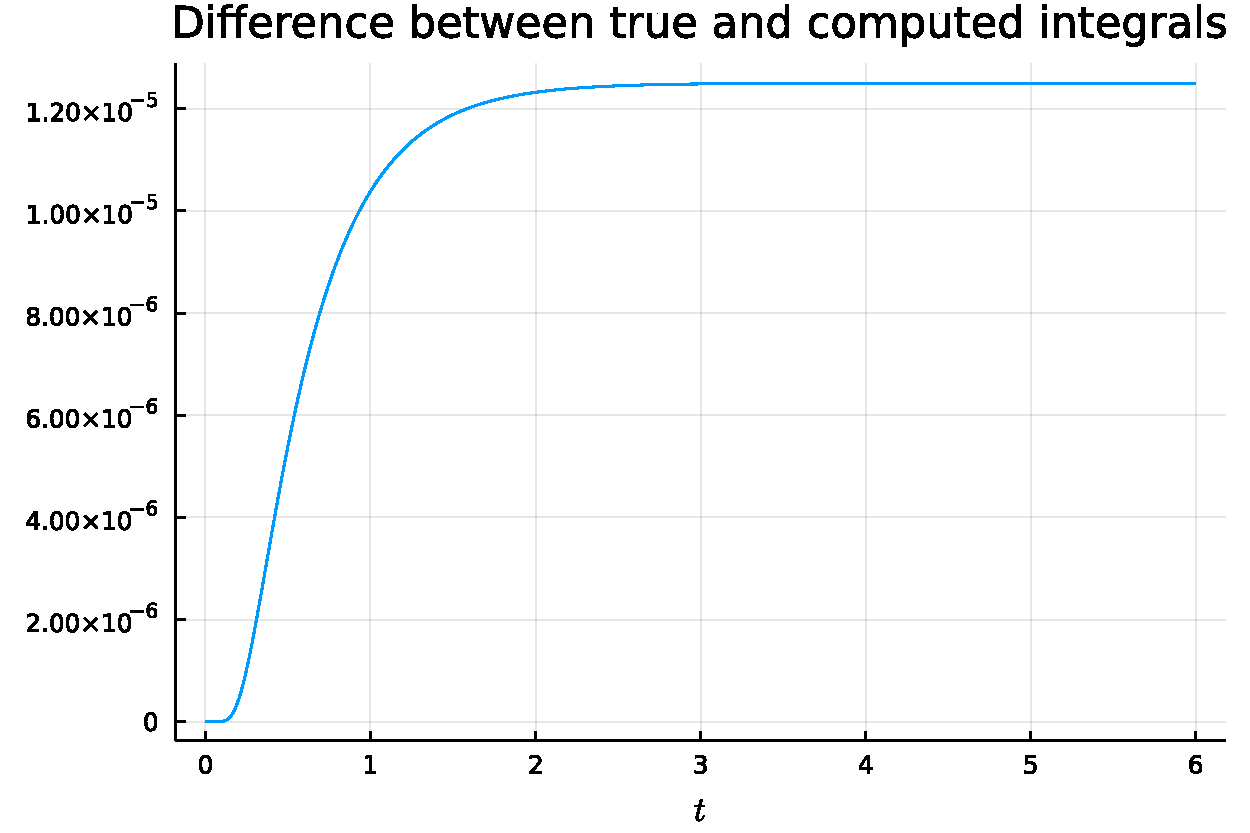
\includegraphics[scale=0.5]{prob3_discrep.pdf}\\
%add discussion here
What we see here is that heat is actually being lost as our computed integral starts at the expected value of $2$ but decreases as time goes on. The likely cause of this is the lack of smoothness in our initial condition. By trying different values of $h=k$, we observe that the heat loss appears to converge to a value that is $\OO(h^2)$\footnote{E.g. choosing $h=k=0.1$ gives a heat loss of $1.2\times 10^{-3}$ instead.} which suggests that this is due to the fact that our TR-BDF-2 method is second order accurate. Since the approximate integral that we are computing is just the $L^1$ grid-norm, we would expect second order accuracy, so this heat loss is consistent. However, the constant on our $\OO(h^2)$ term depends on the smoothness solution at each timestep, and since our initial condition is discontinuous, we expect a large error constant initially that decreases as our solution smooths; this is consistent with how our plot increases dramatically at first before smoothing out. If we instead use a shifted sigmoid function that is similar to $v(x,0)$ but smooth
\[
1-\frac{1}{1+e^{-10(x-2)}}
\]
as our initial condition, we instead find a heat loss that is much closer to machine precision (pictured in the following plot) as the constant should be much smaller.\\
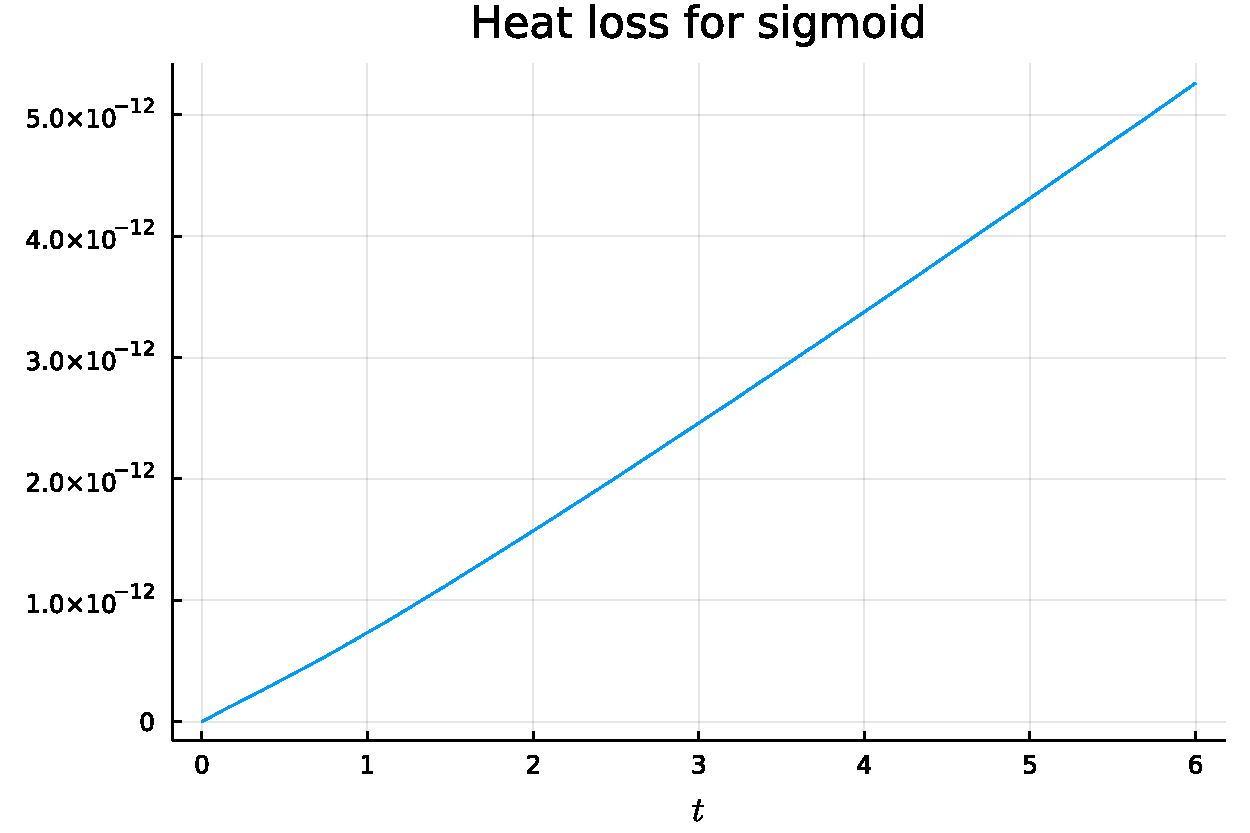
\includegraphics[scale=0.5]{prob3_sigmoid.pdf}\\
However, it is important to note that our sigmoid function does not satisfy our Neumann boundary conditions (but is quite close to doing do), so it is not quite proper to use this as an initial condition for our problem.

%The likely cause of this is the way we have implemented our boundary conditions; by including ghost points, the heat dissipates out to these ghost points, but they are not included in our computed integral.  

\section{Problem 4}
Now, we consider the ODE system
\begin{align*}
	v_t(x,t) &= \kappa v_{xx}(x,t)+  \frac 1 \epsilon \left( g(v(x,t)) - w(x,t) + I_a \right), \quad g(v) = v (\alpha - v) (1-v),\\
	w_t(x,t) &= \beta v(x,t) - \gamma w(x,t)\\
	v_x(a,t) & = 0,\\
	v_x(b,t) & = 0
\end{align*}
for \(x \in (a,b)\). We take $I_a=0$ and Strang split again into the heat equation term and our equation from problem 2. Doing this with the parameters \begin{align*}
	h = 0.02, \quad k = h/10, \quad a = 0, \quad b = 6, \quad \alpha = 0.3,\\
	\beta = 1, \quad \gamma = 1, \quad \kappa = 0.2, \quad \epsilon = 0.001.
\end{align*} and initial data \begin{align*}
	v(x,0) = \begin{cases} 1 &0 \leq x < 1 \\
		0 & \text{otherwise},
	\end{cases} \quad w(x,0) = 0, 
\end{align*}
We solve the problem numerically to time $t=4$ and observe the following computed solution at each integral time. 
\begin{figure}[H]
	\centering
	\begin{subfigure}{0.495\linewidth}
		\centering
		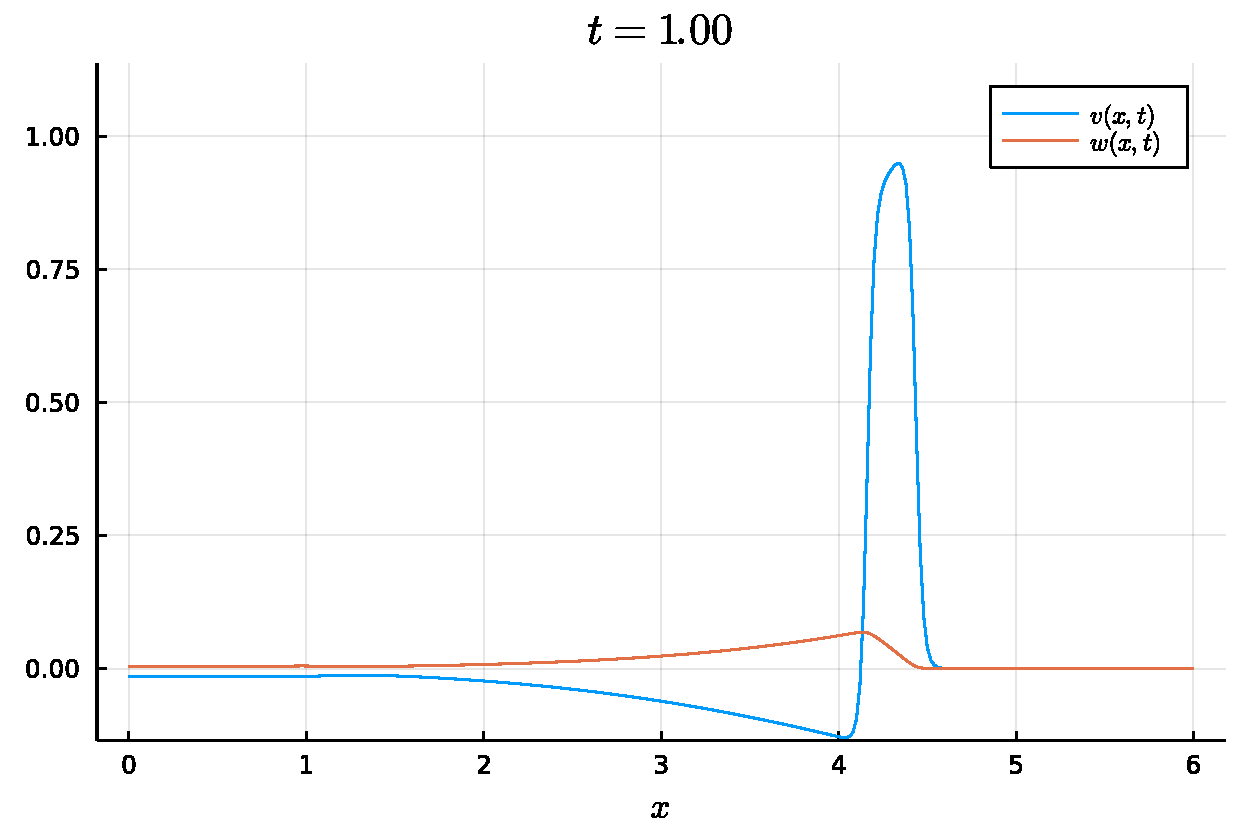
\includegraphics[width=\linewidth]{prob4_t=1.pdf}
	\end{subfigure}
	\begin{subfigure}{0.495\linewidth}
		\centering
		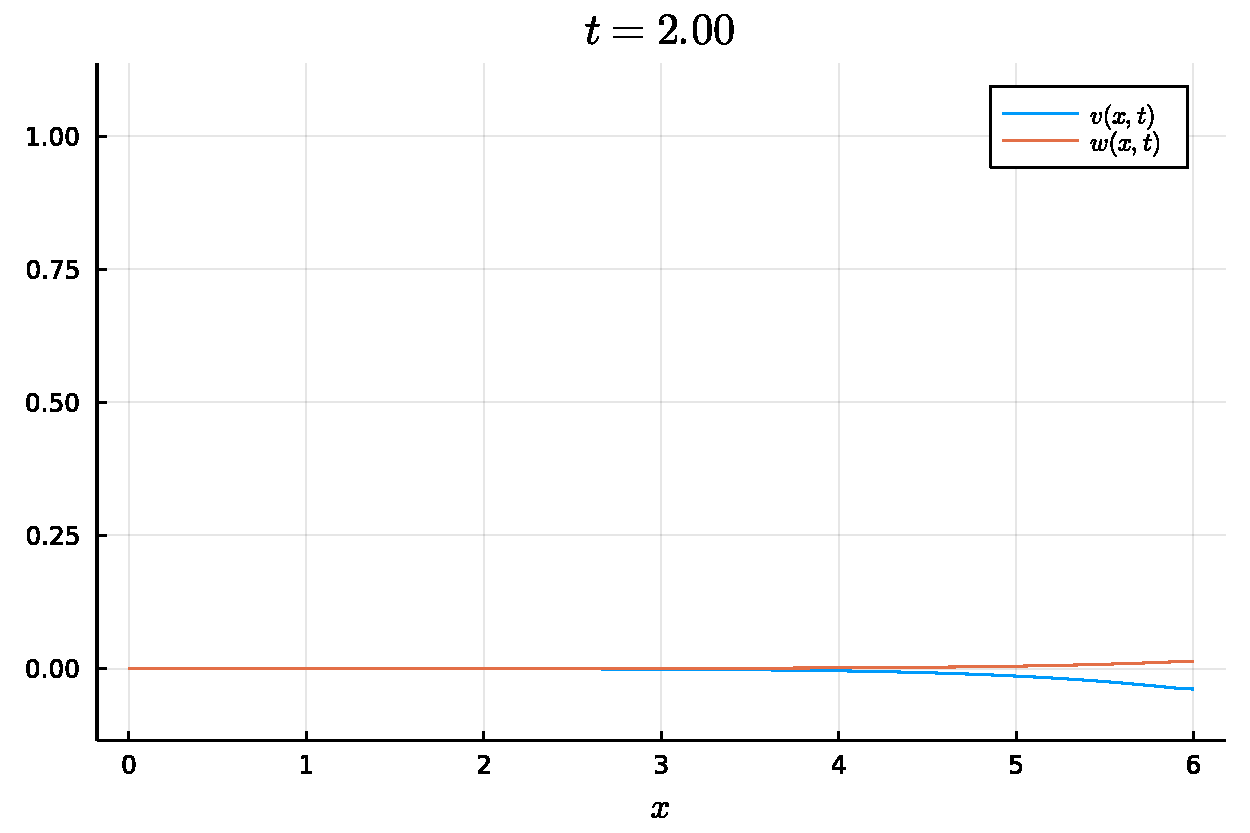
\includegraphics[width=\linewidth]{prob4_t=2.pdf}
	\end{subfigure}
	\begin{subfigure}{0.495\linewidth}
		\centering
		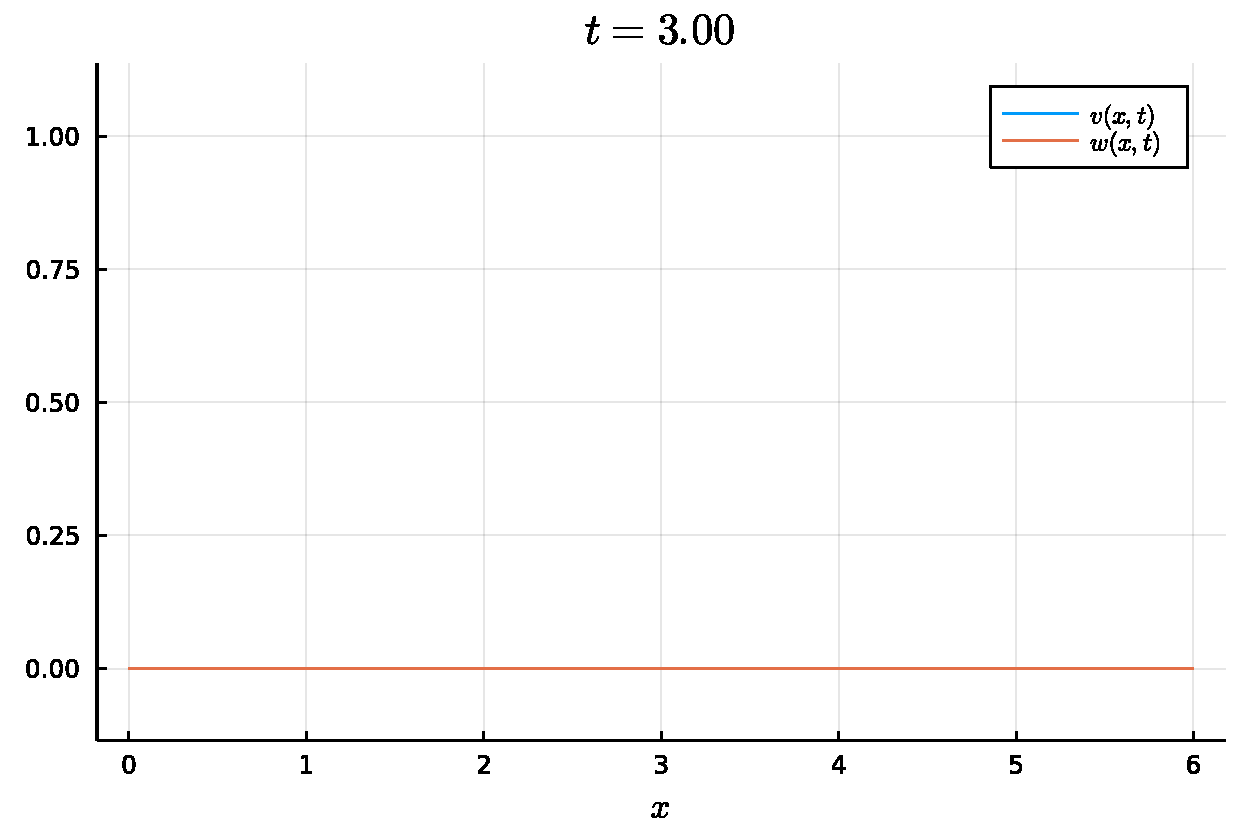
\includegraphics[width=\linewidth]{prob4_t=3.pdf}
	\end{subfigure}
	\begin{subfigure}{0.495\linewidth}
		\centering
		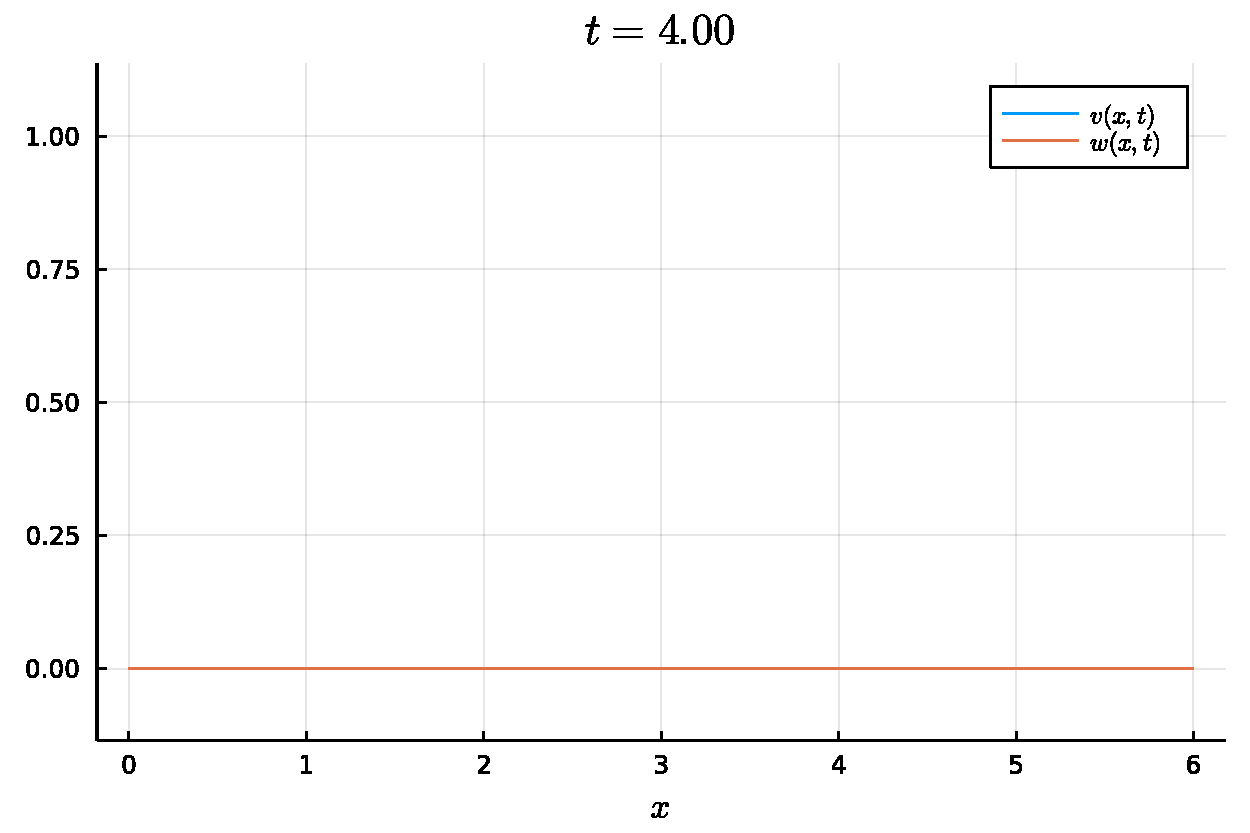
\includegraphics[width=\linewidth]{prob4_t=4.pdf}
	\end{subfigure}
\end{figure}
We also observe the following \href{https://imgur.com/a/XXHi2S8}{gif} of the computed solution.

\section{Problem 5}
Now, we solve the same equation as in problem 4 but instead take 
\begin{align*}
	v(x,0) = 0, \quad w(x,0) = 0, \quad I_a(x) = 0.8 e^{-5x^2}.
\end{align*}
We solve the problem numerically to $t=4$ and observe the following computed solution at each integral time. 
\begin{figure}[H]
	\centering
	\begin{subfigure}{0.495\linewidth}
		\centering
		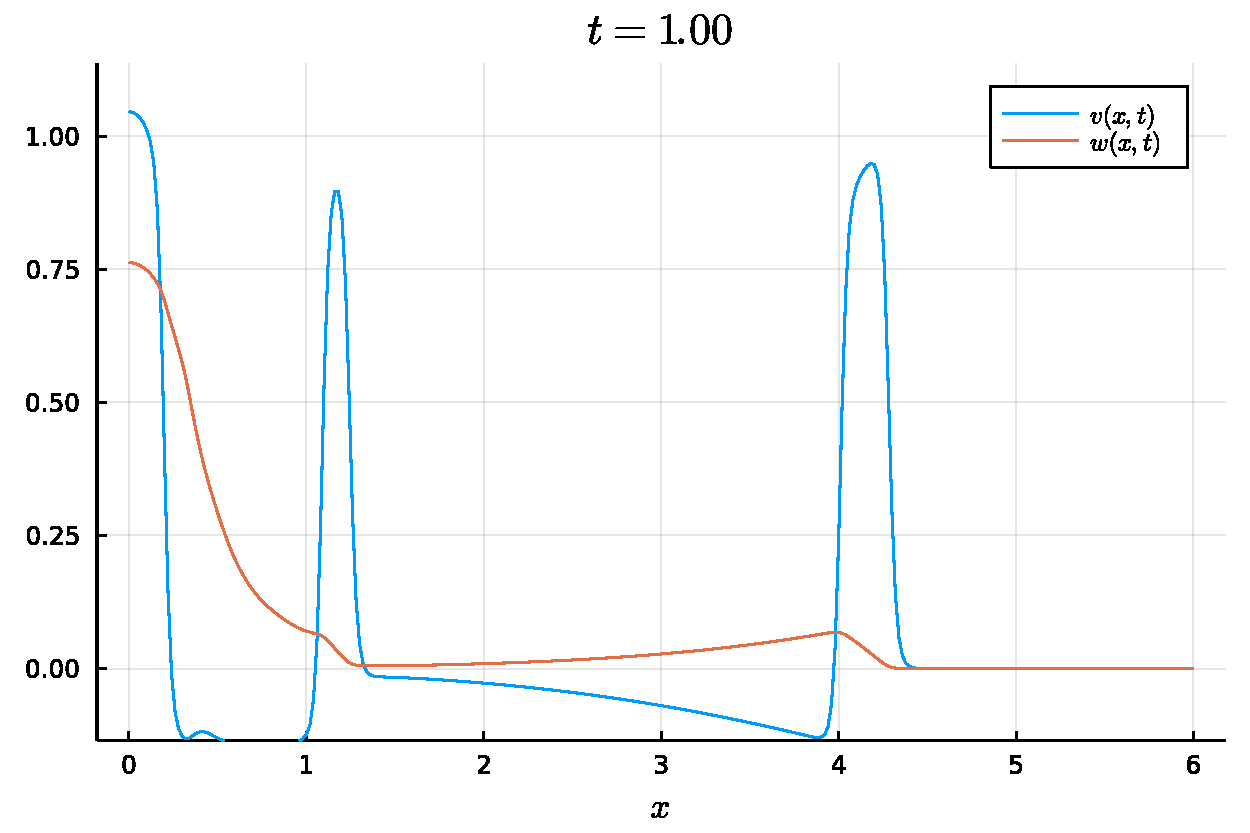
\includegraphics[width=\linewidth]{prob5_t=1.pdf}
	\end{subfigure}
	\begin{subfigure}{0.495\linewidth}
		\centering
		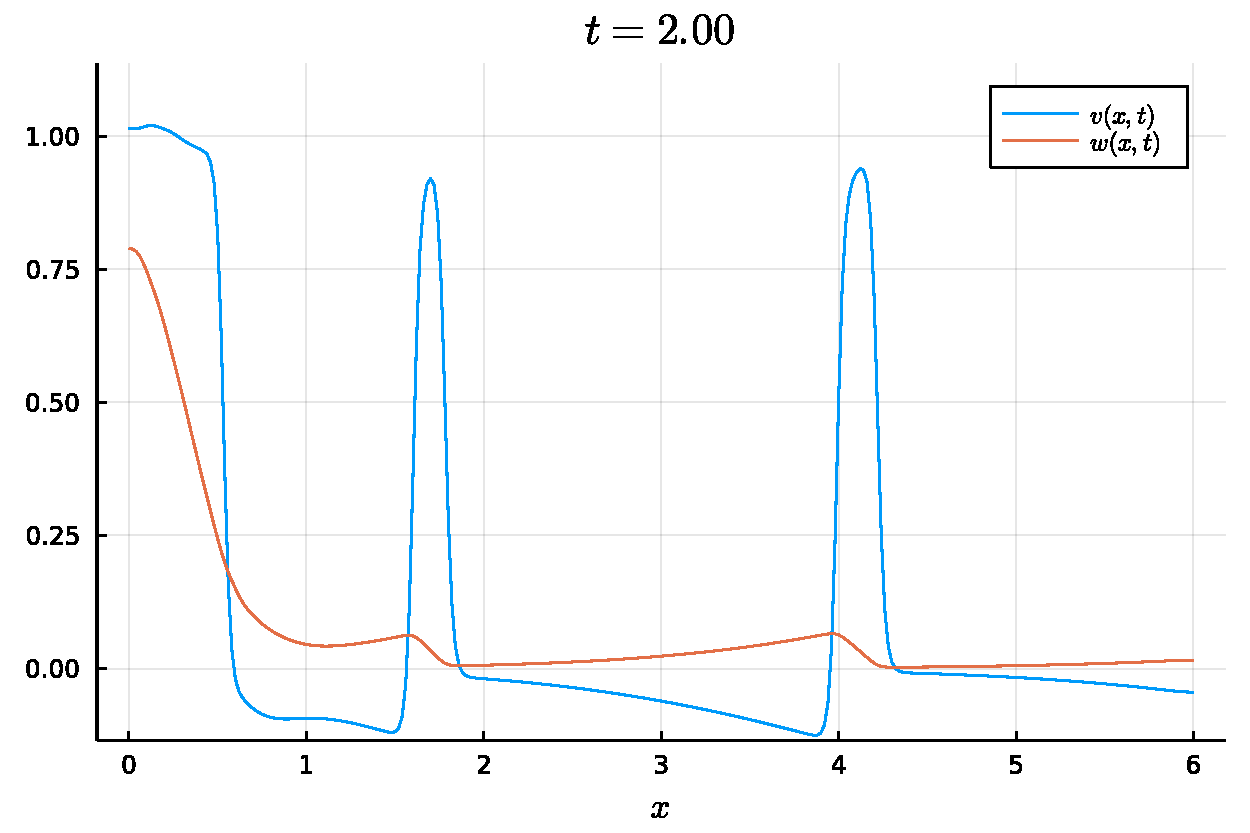
\includegraphics[width=\linewidth]{prob5_t=2.pdf}
	\end{subfigure}
	\begin{subfigure}{0.495\linewidth}
		\centering
		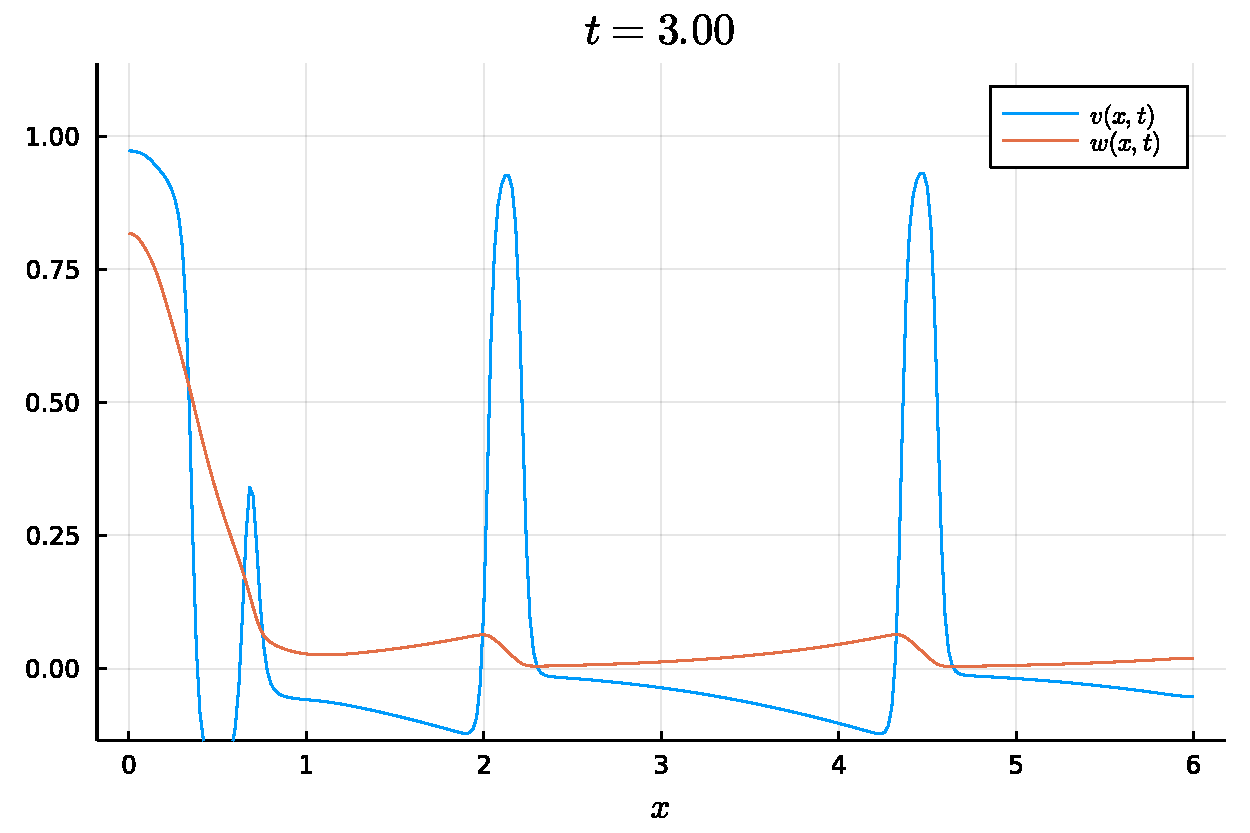
\includegraphics[width=\linewidth]{prob5_t=3.pdf}
	\end{subfigure}
	\begin{subfigure}{0.495\linewidth}
		\centering
		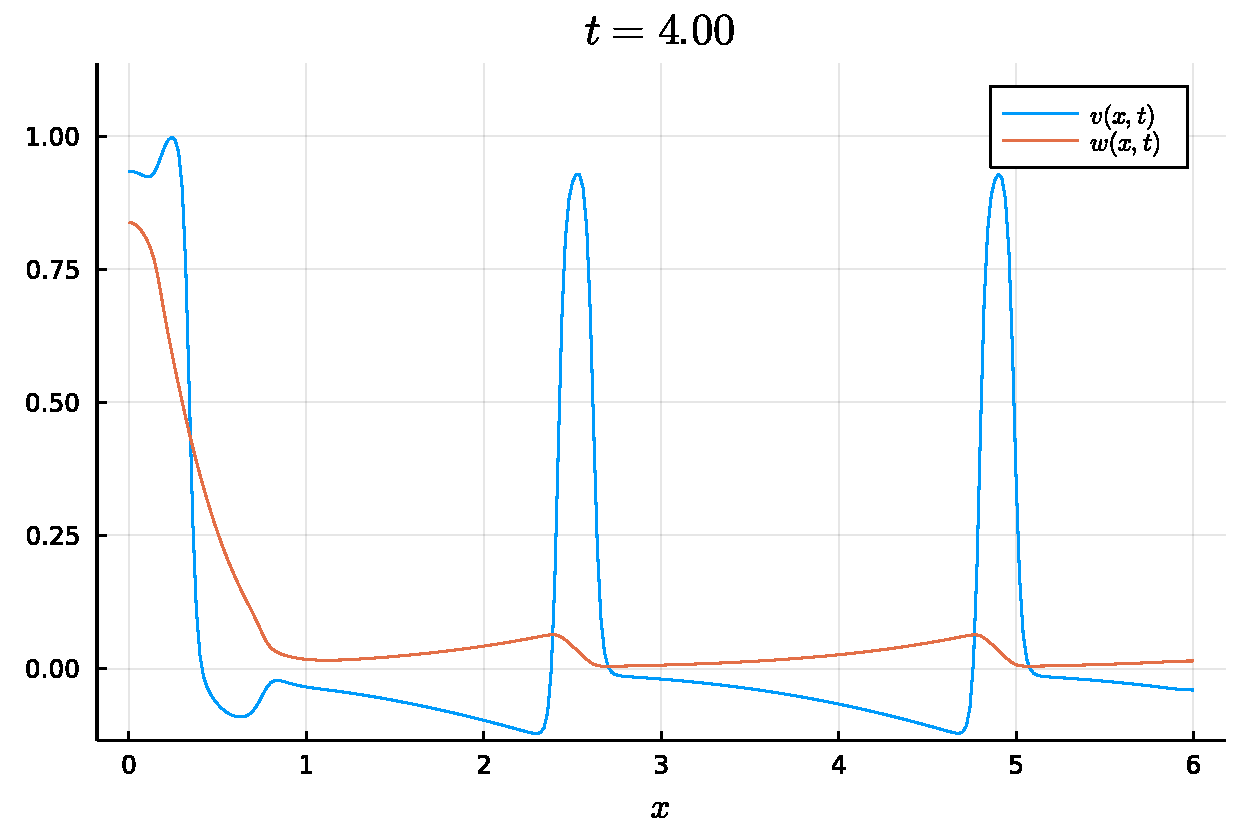
\includegraphics[width=\linewidth]{prob5_t=4.pdf}
	\end{subfigure}
\end{figure}
We also observe the following \href{https://imgur.com/a/wVgVp24}{gif} of the computed solution.

\section{Problem 6}
Now, we consider the extension of problems 4 and 5 to two spatial
dimensions: For \(x \in [a,b], ~y \in [a,b]\): \begin{align*}
	v_t(x,y,t) &= \kappa v_{xx}(x,y,t) + \kappa v_{yy}(x,y,t)+  \frac 1 \epsilon \left( g(v(x,y,t)) - w(x,y,t) + I_a \right), \quad g(v) = v (\alpha - v) (1-v),\\
	w_t(x,y,t) &= \beta v(x,y,t) - \gamma w(x,y,t).
\end{align*}

with initial and boundary data given by

\begin{align*}
	v(x,y,0) = \eta(x,y) = \begin{cases} 1 & x < 2,\\
		0 & \text{otherwise}, \end{cases} \quad w(x,y,0) = 0,\\
	v_x(a,y,t) = v_x(b,y,t) = v_y(x,a,t) = v_y(x,b,t) = 0
\end{align*}
which we solve by Strang splitting in each spatial direction in addition to our prior method. Using parameters \begin{align*}
	a &= 0, \quad b = 12, \quad h = .05, \quad k = h/10, \quad \kappa = 1, \quad \epsilon = 0.01,\\
	\alpha &= 0.1, \quad \beta = 0.5, \quad \gamma = 1, \quad I_a = 0
\end{align*}
and solving to time $t=0.9$, our computed solution for $v$ appears to be a single pulse that
travels across the domain in the positive \(x\)-direction which we display at $t=0$ and $t=0.9$ in the following. 
\begin{figure}[H]
	\centering
	\begin{subfigure}{0.495\linewidth}
		\centering
		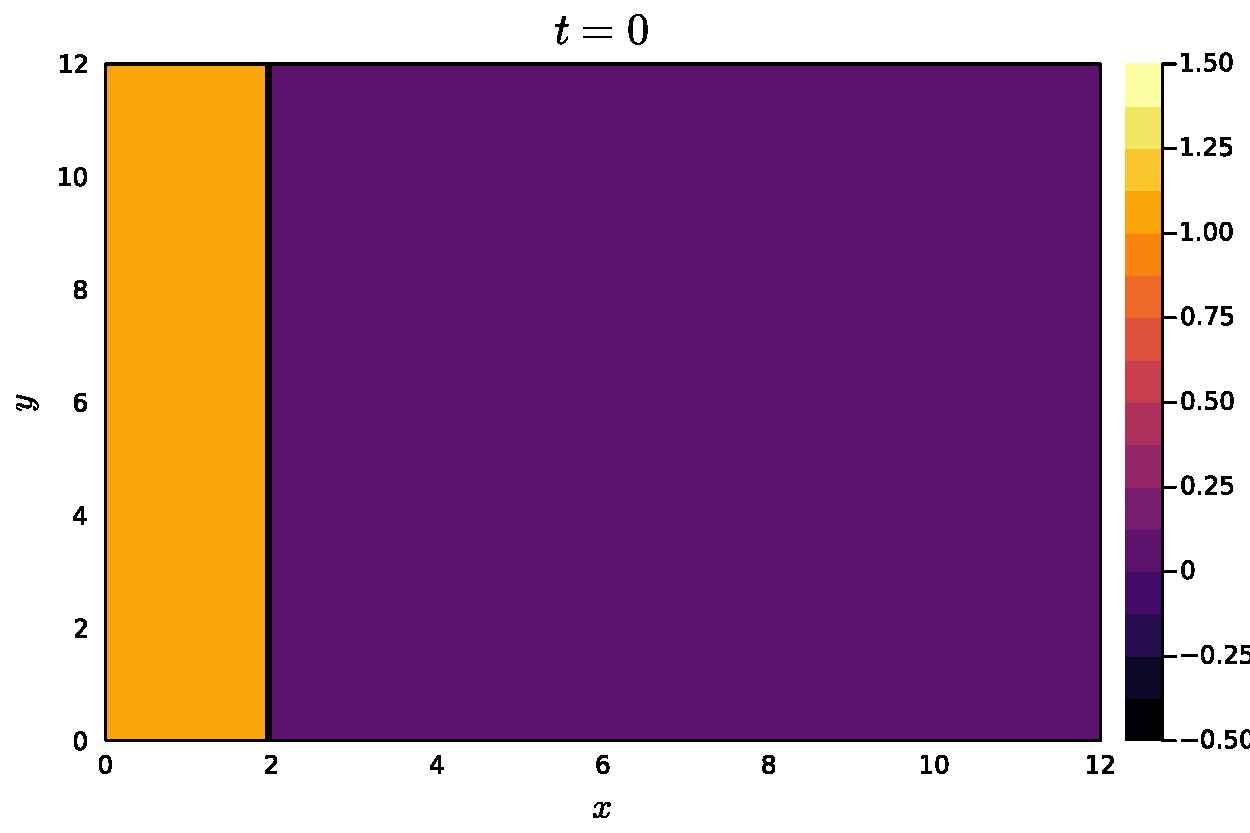
\includegraphics[width=\linewidth]{prob6_t=0.pdf}
	\end{subfigure}
	\begin{subfigure}{0.495\linewidth}
		\centering
		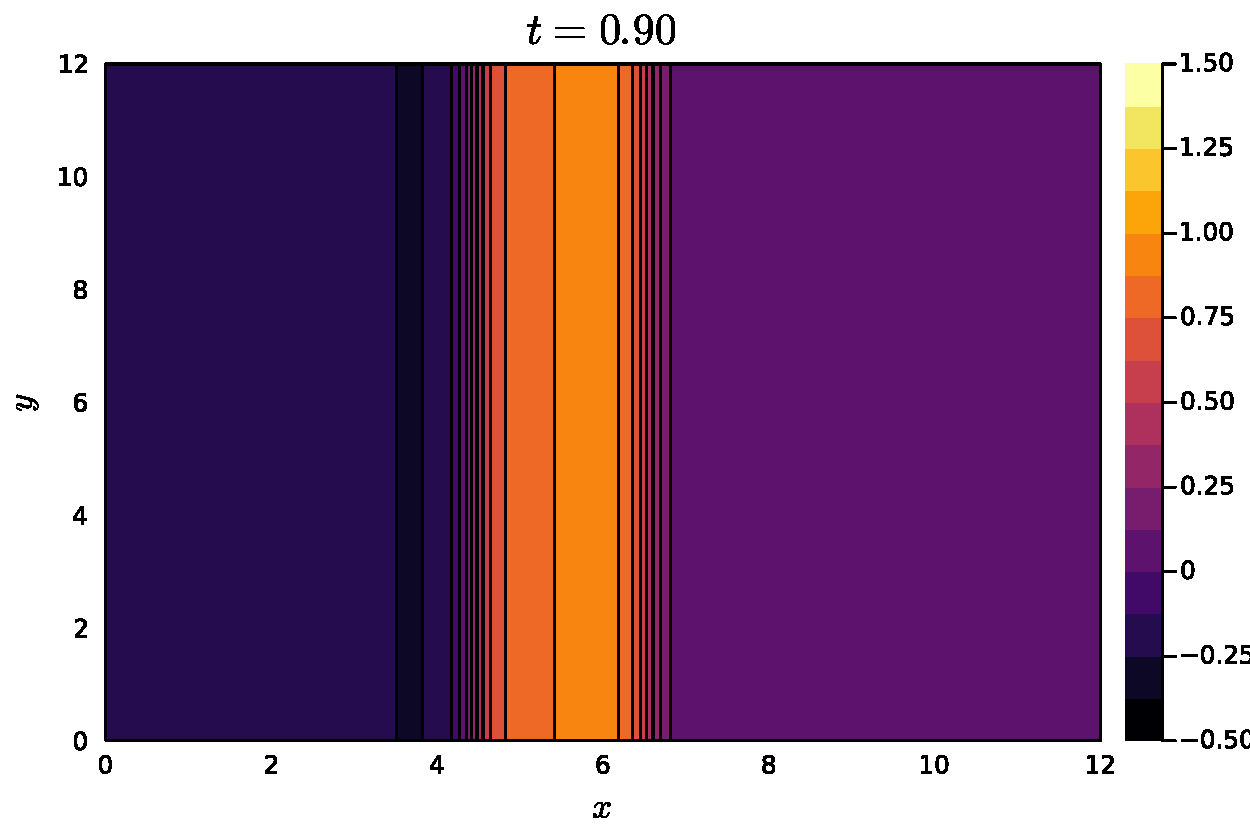
\includegraphics[width=\linewidth]{prob6_t=0.9.pdf}
	\end{subfigure}
\end{figure}
At time $t=0.9$, we zero out all elements of \(V\) with
associated \(y\) coordinates being larger than \(6\) to break the
symmetry in the \(y\)-direction. Solving to time $t=6$, we observe the following computed solution for $v$ at each integral time. 
\begin{figure}[H]
	\centering
	\begin{subfigure}{0.3\linewidth}
		\centering
		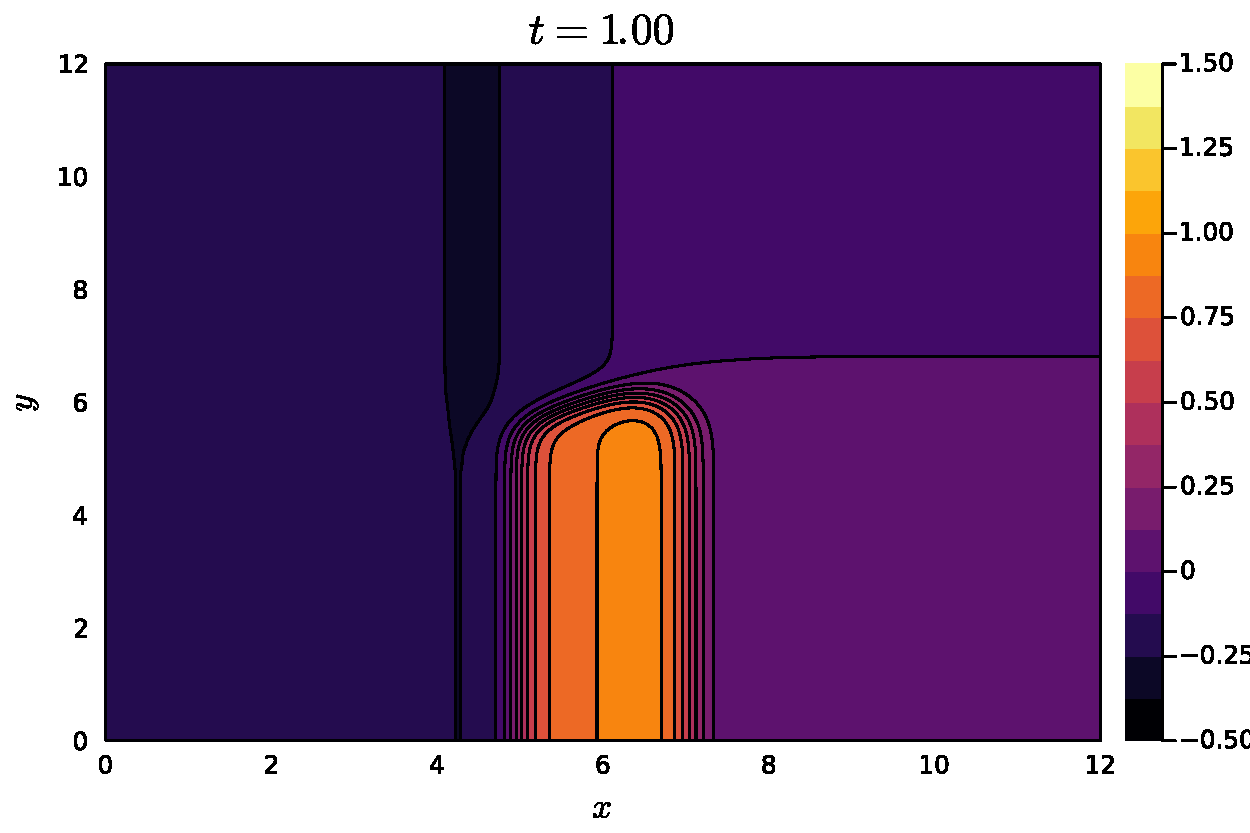
\includegraphics[width=\linewidth]{prob6_t=1.pdf}
	\end{subfigure}
	\begin{subfigure}{0.3\linewidth}
		\centering
		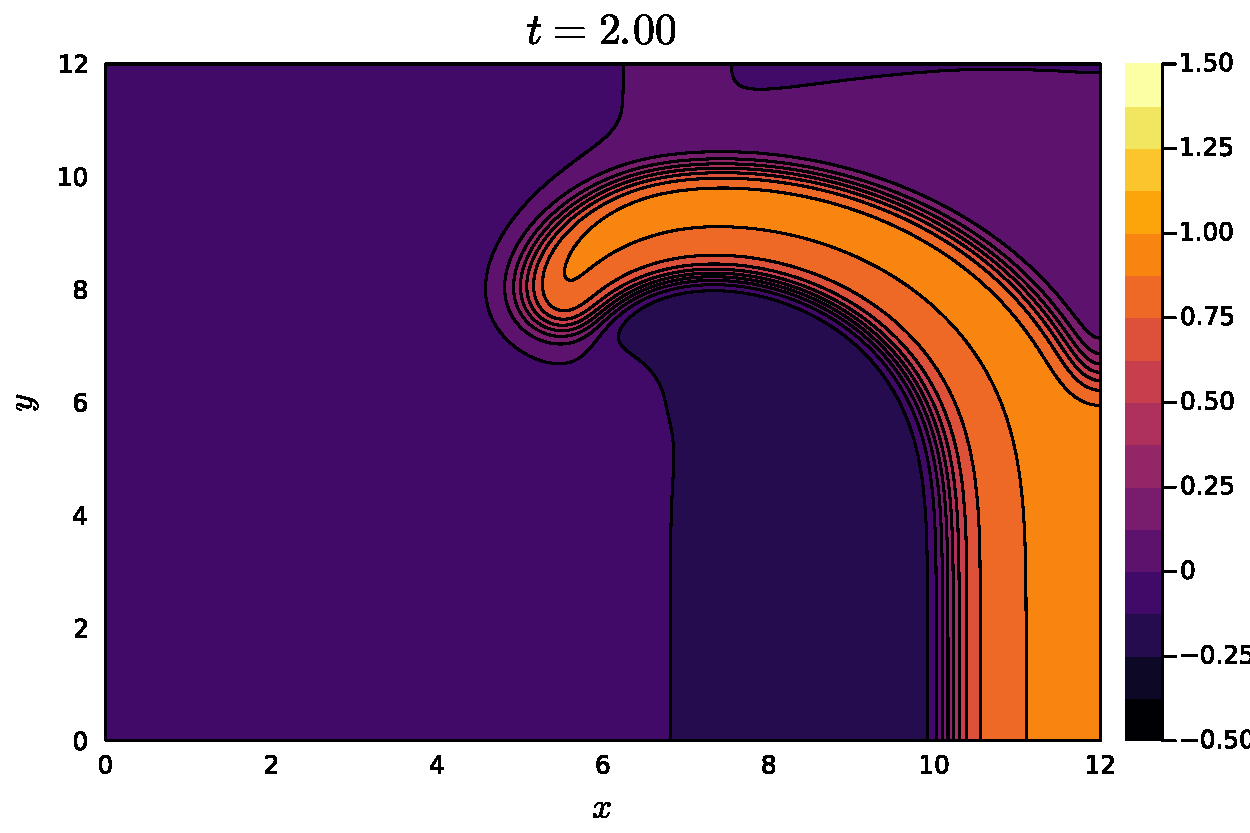
\includegraphics[width=\linewidth]{prob6_t=2.pdf}
	\end{subfigure}
	\begin{subfigure}{0.3\linewidth}
		\centering
		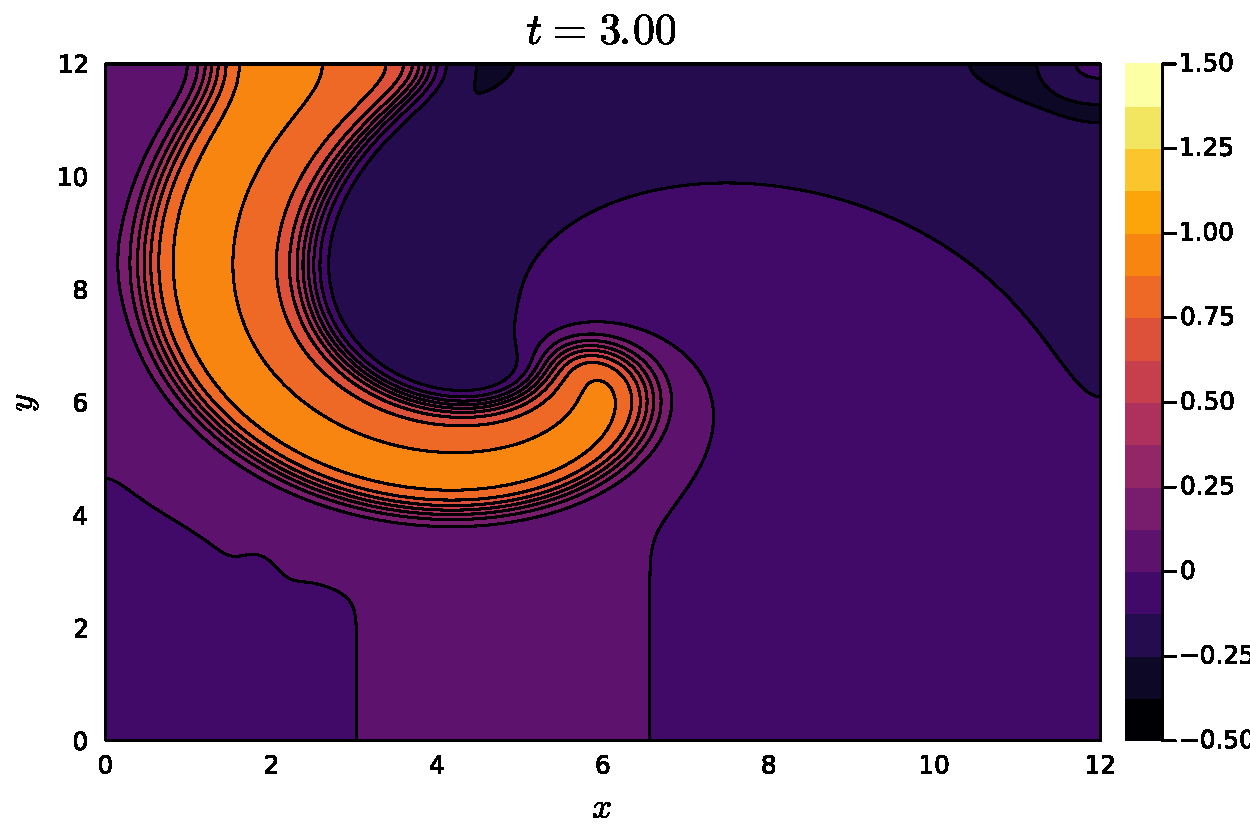
\includegraphics[width=\linewidth]{prob6_t=3.pdf}
	\end{subfigure}
	\begin{subfigure}{0.3\linewidth}
		\centering
		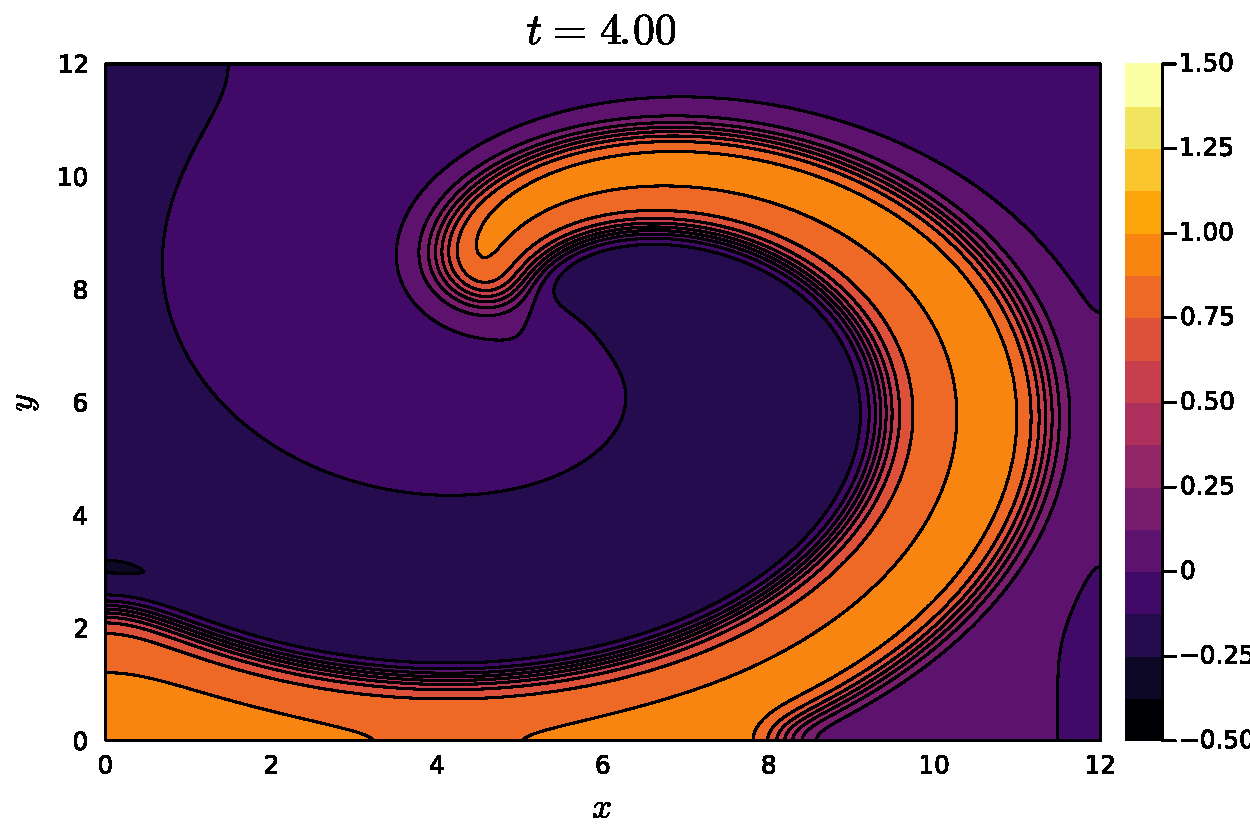
\includegraphics[width=\linewidth]{prob6_t=4.pdf}
	\end{subfigure}
	\begin{subfigure}{0.3\linewidth}
		\centering
		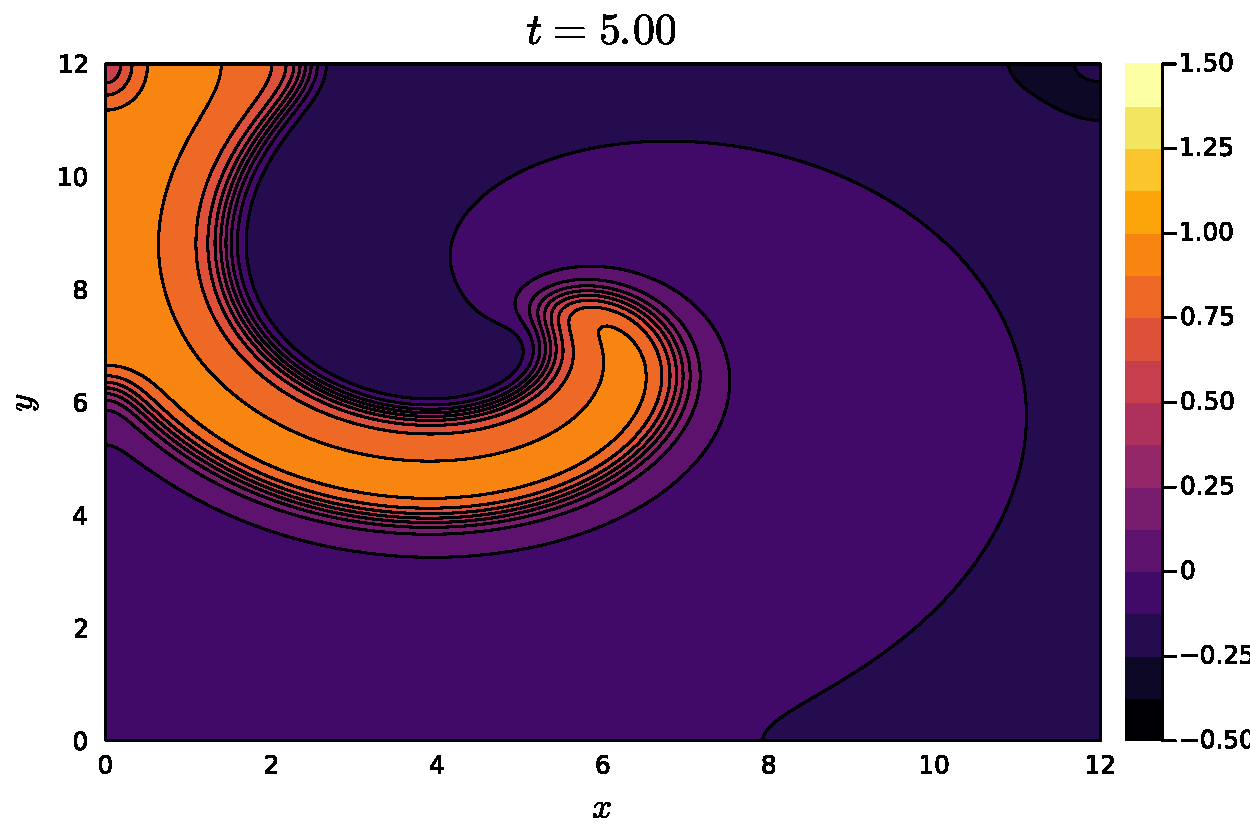
\includegraphics[width=\linewidth]{prob6_t=5.pdf}
	\end{subfigure}
	\begin{subfigure}{0.3\linewidth}
		\centering
		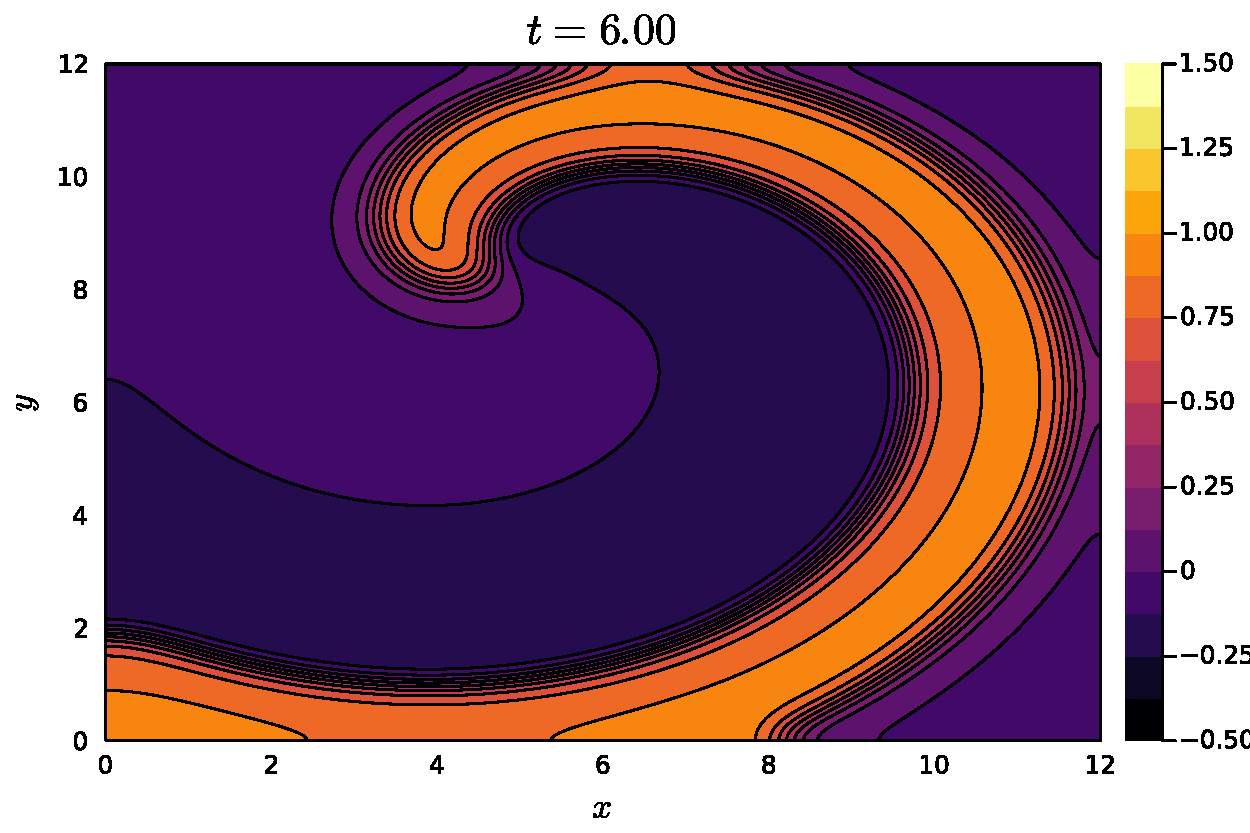
\includegraphics[width=\linewidth]{prob6_t=6.pdf}
	\end{subfigure}
\end{figure}
We also observe the following \href{https://imgur.com/a/skyuaXg}{gif} of the computed solution.

\section{Appendix A}
The following Julia code is used for Problem 1.
\jlinputlisting{Problem1.jl}
The following Julia code is used for Problem 2.
\jlinputlisting{Problem2.jl}
The following Julia code is used for Problem 3.
\jlinputlisting{Problem3.jl}
The following Julia code is used for Problem 4.
\jlinputlisting{Problem4.jl}
The following Julia code is used for Problem 5.
\jlinputlisting{Problem5.jl}
The following Julia code is used for Problem 6.
\jlinputlisting{Problem6.jl}

\end{document}
